%----------------------------------------------------------------------------------------
%	PACKAGES AND THEMES
%----------------------------------------------------------------------------------------
\documentclass{article}

\usepackage{hyperref}
\usepackage{graphicx}
\usepackage[utf8]{vietnam}
\usepackage{geometry}
\usepackage{amsmath}

\geometry{a5paper, top=2cm, left=2cm, right=2cm, bottom=2cm}


\title{Nghiên cứu về đường đoản thời}

\author{Lê Quốc Dũng}

\date{\today}

\begin{document}


\maketitle


\begin{abstract}

Động lực để tác giả viết bài này là sau khi đọc về sự ra đời phép tính vi tích phân cùng vụ tranh cãi đáng xấu hổ trong lịch sử toán học giữa Newton và Leibniz, cùng với bài toán của Johann Bernoulli. 
		
Bài nghiên cứu này được tham khảo nhiều nguồn và là tài liệu học tập cá nhân. Tác giả hy vọng rằng bài nghiên cứu nhỏ này sẽ giúp ích được cho các bạn học sinh, sinh viên đam mê toán và vật lý (mặc dù tác giả không phải dân lý hihi).

\end{abstract}

\tableofcontents

\section{Bối cảnh lịch sử}

Thế kỷ 17 đã chứng kiến một drama có thể gọi là đáng xấu hổ nhất lịch sử toán học. Hai nhà toán học có ảnh hưởng rất lớn lại vướng vào một vụ kiện tụng và tranh cãi khó coi để xem ai là người phát minh ra phép tính vi tích phân. Vâng, chúng ta đang nói đến Newton và Leibniz. Vào thời điểm đó có một nhà toán học xuất sắc thuộc một dòng họ cũng gồm rất nhiều nhân vật xuất sắc đã đưa ra một bài toán đố cho các nhà toán học trên thế giới. Bài toán đó đã chứng minh được ưu thế vượt trội trong phương pháp vi tích phân của Leibniz.
	
Nhà toán học xuất sắc đó là Johann Bernoulli, thuộc dòng họ Bernoulli nổi tiếng. Bài toán đó được phát biểu như sau:
	
\textit{Cho hai điểm A và B nằm trong mặt phẳng thẳng đứng P (A cao hơn B). Hãy 
	xác định đường nối hai điểm A và B và nằm trong mặt phẳng P sao cho một 
	điểm chỉ chịu trọng lực chạy từ A đến B trong thời gian ngắn nhất.}

Chúng ta đã biết rằng đường đi ngắn nhất giữa hai điểm là đoạn thẳng nối hai điểm đó. Tuy nhiên trong bài toán của Johann Bernoulli thì đại lượng ngắn nhất cần tìm không phải khoảng cách giữa hai điểm mà là thời gian di chuyển giữa hai điểm. Mục tiêu cần làm ở bài toán này là xác định đường đi (hay quỹ đạo) thời gian ngắn nhất đó. Do đó bài toán này được gọi là bài toán \textit{đường đoản thời} (brachistochrone curve).

Để giải bài toán này chúng ta cần một định luật cũng về thời gian ngắn nhất. Đó là nguyên lý thời gian ngắn nhất của Fermat và một hệ quả của nó là định luật Snell-Descartes.

\section{Định luật Snell-Descartes}

\begin{figure}[ht]
	\centering
	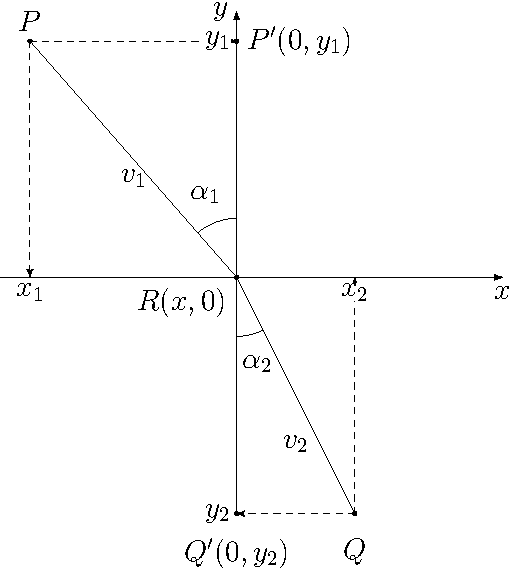
\includegraphics{fermat.pdf}
	\label{snell}
	\caption{Định luật Snell-Descartes}
\end{figure}


Nguyên lý thời gian ngắn nhất của Fermat phát biểu rằng

\textit{Khi ánh sáng truyền từ môi trường này sang môi trường khác thì nó luôn truyền đi theo đường nhanh nhất.}

Hệ quả của nguyên lý của Fermat là định luật Snell-Descartes mà chúng ta thường thấy ở chương trình vật lý ở phổ thông dưới dạng định luật khúc xạ ánh sáng

\begin{equation}
	\frac{\sin \alpha_1}{\sin \alpha_2} = \frac{v_1}{v_2}
\end{equation}
với $\alpha_1$ và $\alpha_2$ lần lượt là góc hợp bởi tia vào và tia ra với pháp tuyến tại điểm tới, $v_1$ và $v_2$ là vận tốc truyền trong môi trường ở nửa trên và nửa dưới $Ox$ (xem hình \ref{snell}).

Để chứng minh định luật trên, ta thấy rằng $v_1$ là vận tốc khi di chuyển từ điểm $P$ tới điểm $R$ nên thời gian $t_1$ đi từ điểm $P$ tới $R$ là
\begin{equation}
	t_1 = \frac{\lvert \overrightarrow{PR} \rvert}{v_1} = \frac{\sqrt{(x - x_1)^2 + y_1^2}}{v_1}
\end{equation}

Lưu ý rằng tia sáng không truyền tới gốc tọa độ $O(0,0)$ mà truyền tới một điểm $R(x,0)$ là vì điểm bắt đầu là $P(x_1, y_1)$ và ánh sáng truyền đi theo đường nhanh nhất (theo nguyên lý Fermat) nên không có gì đảm bảo rằng nó sẽ truyền tới $O(0, 0)$.

Tương tự, thời gian $t_2$ đi từ điểm $R$ tới $Q$ là
\begin{equation}
	t_2 = \frac{\lvert \overrightarrow{RQ} \rvert}{v_2} = \frac{\sqrt{(x - x_2)^2 + y_2^2}}{v_2}
\end{equation}

Kết hợp hai phương trình của $t_1$ và $t_2$ lại thì tổng thời gian di chuyển từ $P$ tới $Q$ biểu diễn theo $x$ là
\begin{equation}
	T(x) = t_1 + t_2 = \frac{\sqrt{(x - x_1)^2 + y_1^2}}{v_1} + \frac{\sqrt{(x - x_2)^2 + y_2^2}}{v_2}
\end{equation}

Đạo hàm theo $x$ ta có
\begin{equation}
	T'(x) = \frac{x - x_1}{v_1 \sqrt{(x - x_1)^2 + y_1^2}} + \frac{x - x_2}{v_2 \sqrt{(x - x_2)^2 + y_2^2}}
\end{equation}

Để ý rằng $x > x_1$ nên $x - x_1 = \lvert \overrightarrow{PP'} \rvert$. Tương tự $x_2 - x = \lvert \overrightarrow{QQ'} \rvert$. Để tìm cực trị ta cho đạo hàm bằng 0 rồi tính đạo hàm cấp 2. Ta có

\[T'(x) = 0 \Leftrightarrow \frac{\lvert \overrightarrow{PP'} \rvert}{v_1 \lvert \overrightarrow{PR} \rvert} - \frac{\lvert \overrightarrow{QQ'} \rvert}{v_2 \lvert \overrightarrow{RQ} \rvert} = 0 \Leftrightarrow \frac{\sin \alpha_1}{v_1} - \frac{\sin \alpha_2}{v_2} = 0\]

Như vậy $\dfrac{\sin \alpha_1}{v_1} = \dfrac{\sin \alpha_2}{v_2}$. Đạo hàm cấp 2 tương ứng là

\[ T''(x) = \frac{y_1^2}{v_1 ((x - x_1)^2 + y_1^2)} + \frac{y_2^2}{v_2 ((x - x_2)^2 + y_2^2)} > 0 \]

Do đó $x$ thỏa $T'(x) = 0$ ở trên là cực tiểu và định luật Snell-Descartes được chứng minh.

\section{Đường cong Cycloid}

Đáp án cho bài toán mà Johann Bernoulli đặt ra là đường cong Cycloid. Sau đây sẽ trình bày cách giải bài toán của Johann Bernoulli.

\begin{figure}[ht]
	\centering
	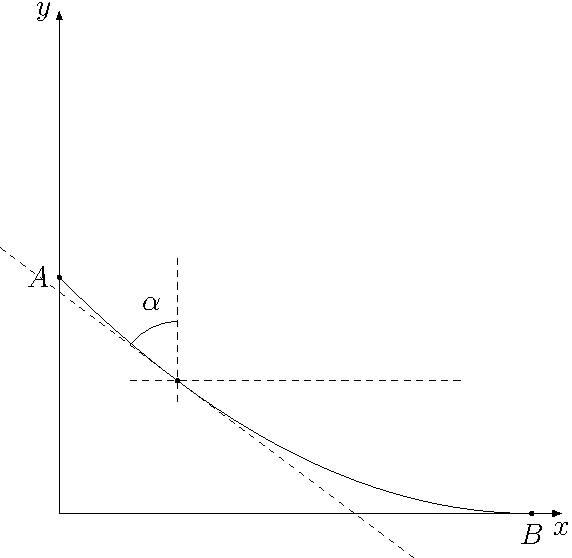
\includegraphics{brachistochrone.pdf}
	\label{cycloid:im1}
\end{figure}

Phương của vận tốc tức thời tại một điểm khi một vật đi theo một quỹ đạo đường cong là tiếp tuyến với đường cong tại điểm đó. Khi đó góc $\alpha$ trong định luật Snell-Descartes sẽ có liên hệ với hệ số góc của tiếp tuyến với đường cong. Nói rõ hơn, góc hợp bởi tiếp tuyến và trục $Ox$ là $\alpha + \dfrac{\pi}{2}$ và hệ số góc của tiếp tuyến là $\tan \Bigl(\alpha + \dfrac{\pi}{2}\Bigr) = \dfrac{dy}{dx}$ (hình \ref{cycloid:im1}).

Ta có $\tan \Bigl( \alpha + \dfrac{\pi}{2} \Bigr) = -\cot \alpha$ và $1 + \cot^2 \alpha = \dfrac{1}{\sin^2 \alpha}$ nên 

\begin{equation}
	\dfrac{1}{\sin^2 \alpha} = 1 + \cot^2 \alpha = 1 + \Bigl(\dfrac{dy}{dx}\Bigl)^2
\end{equation}

Giả sử tọa độ của $A$ là $(x_0, y_0)$. Khi một điểm di chuyển từ $A$ tới $B$, gọi $(x, y)$ là tọa độ của điểm đó trên đường cong. Theo định luật bảo toàn cơ năng thì 

\begin{equation*}
	m g y_0 = \frac{1}{2} m v^2 + m g y
\end{equation*}
với $v$ là vận tốc tức thời tại điểm $(x, y)$ và $mgy$ là thế năng tại điểm đó. Như vậy ta có 

\begin{equation}
	v^2 = 2 g (-y + y_0)
\end{equation}

Theo định luật Snell-Descartes thì $\dfrac{v}{\sin \alpha}$ là một hằng số khi nằm trong cùng môi trường. Do đó tồn tại số $r$ cố định sao cho $\dfrac{v^2}{\sin^2 \alpha} = 4 g r$. Từ hai biểu thức của $v^2$ và $\dfrac{1}{\sin^2 \alpha}$ ở trên ta có

\begin{equation}
	\frac{v^2}{\sin^2 \alpha} = 2 g (-y + y_0) \Bigl( 1 + \Bigl(\frac{dy}{dx}\Bigr)^2 \Bigr) = 4 g r
\end{equation}

Suy ra

\begin{equation}
	\Big(\frac{dy}{dx}\Big)^2 = \frac{2 r}{y_0 - y} - 1
	\label{diff:eq1}
\end{equation}

Tới đây ta thấy rằng bậc của $dy$ và $dx$ ở vế trái là giống nhau, trong khi vế phải chỉ có $y$ mà không có $x$. Do đó "bắt chước" cách đổi biến của đường tròn, đặt

\[ \begin{cases}
	x = a \theta + b \cos \theta \\
	y = c + d \sin \theta
\end{cases} \]
với $a$, $b$, $c$, $d$ là các số thực cần tìm, $\theta$ là góc hợp bởi $Oy$ và đoạn thẳng nối tâm $O$ và điểm trên đường cong (theo góc $\alpha$). Lưu ý rằng khi thay $\theta = 0$ và $\theta = \pi / 2$ vào hai phương trình trên ta phải thu được hai điểm trên hai trục tọa độ.

Lấy vi phân hai phương trình trên ta có

\[ \begin{cases}
	dx = a - b \sin \theta \, d \theta \\ dy = d \cos \theta \, d \theta
\end{cases}\]

Thay vào phương trình \ref{diff:eq1} ta được

\begin{equation*}
	\frac{d^2 \cos^2 \theta}{(a - b \sin \theta)^2} = \frac{2 r}{y_0 - c - d \sin \theta} - 1 = \frac{2 r - y_0 + c + d \sin \theta}{y_0 - c - d \sin \theta}
\end{equation*}

Do $\cos^2 \theta = 1 - \sin^2 \theta = (1 - \sin \theta)(1 + \sin \theta)$ nên ta muốn chọn $a$ và $b$ có thể rút gọn được cho tử số. 

\textbf{Trường hợp 1}. $a = b$, ta thu được

\begin{equation*}
	\frac{d^2 (1 + \sin \theta)}{a^2 (1 - \sin \theta)} = \frac{(2 r - y_0 + c) + d \sin \theta}{(y_0 - c) - d \sin \theta}
\end{equation*}

Ta sẽ muốn đồng nhất hệ số tự do và hệ số trước $\sin \theta$ để dễ tính toán sau này. Do đó một cách chọn đơn giản là $2 r - y_0 + c = d$ và $y_0 - c = d$. Suy ra $r = d$. Thu gọn phương trình ta được

\begin{equation*}
	\frac{d^2 (1 + \sin \theta)}{a^2 (1 - \sin \theta)} = \frac{1 + \sin \theta}{1 - \sin \theta}
\end{equation*}

Như vậy $a^2 = d^2$ nên $a = d$ hoặc $a = -d$. Ta xét trường hợp $a = d$, trường hợp $a = -d$ cũng cho kết quả tương tự (không thỏa mãn). 

Ta có  $a = b = d = r$ và $c = y_0 - d = y_0 - r$. Phương trình đường cong trong tọa độ cực sẽ là

\begin{equation*}
	\begin{cases}
		x = r(\theta + \cos \theta) \\ y = (y_0 - r) + r \sin \theta
	\end{cases}
\end{equation*}

Với $\theta = 0$ thì $(x, y) = (r, y_0 - r$. Với $\theta = \pi / 2$ thì $(x, y) = (\pi r / 2, y_0)$.

Tới đây chúng ta có thể thêm bớt một hằng số để "kéo" các tọa độ về trục. 

Ta đưa tọa độ khi $\theta = 0$ về $Oy$ thì $x' = x - r$. Tương tự tọa độ khi $\theta = \pi / 2$ sẽ về $Ox$ nên $y' = y - y_0$. Như vậy tọa độ (mới) cho hai trường hợp $\theta$ là $(0, -r)$ và $(\pi r / 2 - 1, 0)$ nhưng vì $r$ là số dương (bán kính) nên $(0, -r)$ nằm dưới trục $Ox$, không phù hợp với hình vẽ.

\textbf{Trường hợp 2}. $a = -b$, ta thu được

\begin{equation*}
	\frac{d^2 (1 - \sin\theta)}{a^2 (1 + \sin\theta)} = \frac{(2r - y_0 + c) + d \sin\theta}{(y_0 - c) - d \sin\theta}
\end{equation*}

Tương tự, để đồng nhất và rút gọn hệ số cho hợp với bên vế trái ta chọn $2r - y_0 + c = -d$ và $y_0 - c = -d$. Suy ra $d = -r$. Thu gọn phương trình ta được

\begin{equation*}
	\frac{d^2 (1 - \sin\theta)}{a^2 (1 + \sin\theta)} = \frac{1 - \sin\theta}{1 + \sin\theta}
\end{equation*}

Như vậy $a^2 = d^2$ nên $a = d$ hoặc $a = -d$ Ta xét trường hợp $a = -d$.

Khi đó $a = -b = -d = r$ và $c = y_0 + d = y_0 - r$. Phương trình đường cong trong tọa độ cực sẽ là 

\begin{equation*}
	\begin{cases}
		x = r (\theta - \cos\theta) \\
		y = (y_0 - r) - r \sin\theta
	\end{cases}
\end{equation*}

Với $\theta = 0$ thì $(x, y) = (-r, y_0)$. Với $\theta = \pi / 2$ thì $(x, y) = (r (\pi / 2 - 1), y_0 - 2r)$.

Tới đây ta cũng thêm bớt một hằng số vào hoành độ và tung độ để "kéo" các tọa độ về trục.

Ta đưa tọa độ khi $\theta = 0$ về $Oy$ thì $x' = x + r$. Tương tự ta đưa tọa độ khi $\theta = \pi / 2$ về $Ox$ thì $y' = y - y_0 + 2r$. Khi đó tọa độ (mới) là $(0, 2r)$ và $(\pi r / 2, 0)$. Điều này phù hợp với yêu cầu bài toán và tương đương với phương trình trong tọa độ cực 

\begin{equation}
	\begin{cases}
		x = r (\theta - \cos\theta) + r = r (1 + \theta - \cos\theta) \\
		y = (y_0 - r) - r \sin\theta - (y_0 - 2r) = r (1 - \sin\theta)
	\end{cases}, 0 \leq \theta \leq \frac{\pi}{2}
\end{equation}

Đây chính là kết quả cần tìm. Thêm nữa vị trí ban đầu của vật là $(0, y_0)$ và tọa độ theo phương trình là $(0, 2r)$ nên suy ra $y_0 = 2r$.

\section{Phương trình phụ thuộc thời gian}

Trong phương trình đường cong có sự tham gia của bán kính $r$ cố định và góc quét $\theta$. Chúng ta cần mối liên hệ giữa các phương trình theo thời gian.

Nhắc lại, vận tốc tức thời tại một điểm có phương trùng với tiếp tuyến với đường cong tại điểm đó. Do đó $v = \dfrac{\sqrt{(dy)^2 + (dx)^2}}{dt}$ xác định vận tốc tức thời với quãng đường là $(dy)^2 + (dx)^2$ là bình phương khoảng cách trong mặt phẳng. Từ đây suy ra

\begin{align*}
	v^2 = \Bigl(\frac{dy}{dt}\Bigr)^2 + \Bigl(\frac{dx}{dt}\Bigr)^2 = r^2 \cos^2 \theta \Bigl( \frac{d \theta}{dt} \Bigr)^2 + r^2 (1 + \sin \theta)^2 \Bigl( \frac{d \theta}{dt} \Bigr)^2 \\ = 2 r^2 (1 + \sin \theta) \Bigl( \frac{d \theta}{dt} \Bigr)^2
\end{align*}

Từ bên trên và $y_0 = 2r$ ta có \[v^2 = 2 g (y_0 - y) = 2 g (y_0 - r + r \sin \theta) = 2 g r ( 1 + \sin \theta)\]

Suy ra

\begin{equation*}
	2 r^2 (1 + \sin \theta) \Bigl( \frac{d \theta}{dt} \Bigr)^2 = 2 g r (1 + \sin \theta)
\end{equation*}
Hay

\begin{equation}
	\Bigl(\frac{d \theta}{dt}\Bigr)^2 = \frac{g}{r} \Rightarrow \frac{d \theta}{dt} = \sqrt{\frac{g}{r}} = \text{const}
\end{equation}

Như vậy $\theta = \sqrt{\dfrac{g}{r}} t = \omega t$. Ở đây $t$ là thời gian tính từ lúc bắt đầu thả vật từ điểm $A$. Cuối cùng phương trình phụ thuộc thời gian của đường cong Cycloid là

\begin{equation}
	\begin{cases}
		x = r (1 + \omega t - \cos \omega t) \\ y = r (1 - \sin \omega t)
	\end{cases}
\end{equation}

Trong đó, $r$ là bán kính cố định (bằng nửa độ cao ban đầu $y_0$ của vật), $\omega = \frac{g}{r}$ là tần số góc, $y_0$ là độ cao ban đầu của vật (tung độ điểm $A$).

\begin{thebibliography}{9}
	\bibitem{article}
	Miguel A. Lerma, \emph{A simple derivation of the equation for the brachistochrone curve}, \url{https://sites.math.northwestern.edu/~mlerma/papers-and-preprints/brachistochrone.pdf}
	
	\bibitem{article}
	Lê Quang Ánh, \emph{Gia đình Bernoulli: một dòng họ Toán học}, trang 7 về Johann Bernoulli, \url{https://rosetta.vn/lequanganh/gia-dinh-bernoulli-mot-dong-ho-toan-hoc/}.
\end{thebibliography}
\end{document}